\RequirePackage{luatex85}
\documentclass[border=1pt]{standalone}
\usepackage{tikz}
\usetikzlibrary{arrows}
%%%%%%%%%%%%%%%%%%%%%%%%%%%%%%%%%%%%%%%%%%%%%%%%%%%%%%%%%%%%%%%%%%%%%%%%%%%%%%%%
%%%%%%%%%%%%%%%%%%%%                 colours                %%%%%%%%%%%%%%%%%%%% 
%%%%%%%%%%%%%%%%%%%%%%%%%%%%%%%%%%%%%%%%%%%%%%%%%%%%%%%%%%%%%%%%%%%%%%%%%%%%%%%%

\definecolor{tugreen}{RGB}{128, 186, 38}
\definecolor{tucitron}{RGB}{249, 219, 0}



%%%%%%%%%%%%%%%%%%%%%%%%%%%%%%%%%%%%%%%%%%%%%%%%%%%%%%%%%%%%%%%%%%%%%%%%%%%%%%%%
%%%%%%%%%%%%%%%%%%%%                 Boxes                  %%%%%%%%%%%%%%%%%%%% 
%%%%%%%%%%%%%%%%%%%%%%%%%%%%%%%%%%%%%%%%%%%%%%%%%%%%%%%%%%%%%%%%%%%%%%%%%%%%%%%%
\tikzstyle{normalBox} = [shape=rectangle, draw=black, text=black, thick, 	
	align=center, fill=white]

\tikzstyle{roundBox} = [shape=circle, draw=black, text=black, thick, 	
	align=center, fill=white]

\tikzstyle{alternBox} = [shape=rectangle, text=white, thick, align=center, 
	fill=black, rounded corners]


%%%%%%%%%%%%%%%%%%%%%%%%%%%%%%%%%%%%%%%%%%%%%%%%%%%%%%%%%%%%%%%%%%%%%%%%%%%%%%%%
%%%%%%%%%%%%%%%%%%%%                 Arrows                 %%%%%%%%%%%%%%%%%%%% 
%%%%%%%%%%%%%%%%%%%%%%%%%%%%%%%%%%%%%%%%%%%%%%%%%%%%%%%%%%%%%%%%%%%%%%%%%%%%%%%%

\tikzstyle{normalArrow} = [thick,->,>=stealth, draw=black]

\usepackage[utf8]{inputenc}
\usepackage[T1]{fontenc}
\usepackage[sfdefault]{FiraSans}

\tikzstyle{AlternBox} = [alternBox, text width =0.7cm]
\tikzstyle{NormalBox} = [normalBox, text width =1cm, minimum height=0.5cm]
\begin{document}
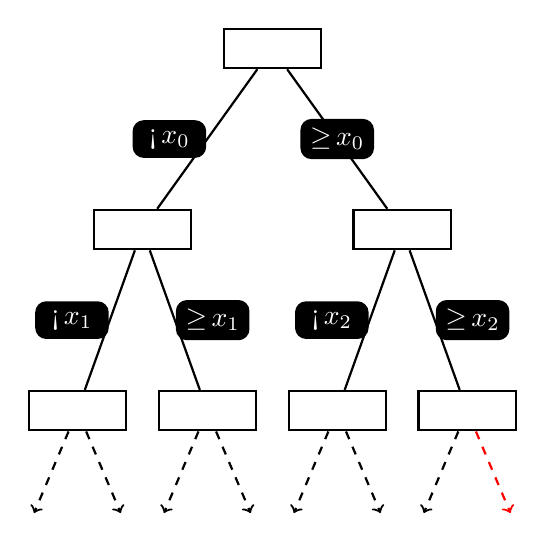
\begin{tikzpicture}[
	edge from parent/.style = {thick, draw},
	level distance = 23mm , level/.style ={sibling distance = 33mm/#1}
  ]
  \node[NormalBox] {}
  child { node[NormalBox] {}
  	child{ node[NormalBox] {}
		child[level distance = 13mm, dashed, ->]
		child[level distance = 13mm, dashed, ->]
		edge from parent node[AlternBox, left] {<\,$x_1$}
  	}
  	child { node[NormalBox] {}
		child[level distance = 13mm, dashed, ->]
		child[level distance = 13mm, dashed, ->]
		edge from parent node[AlternBox, right] {$\ge$\,$x_1$}
 	}
	edge from parent node[AlternBox, left] {<\,$x_0$}
  }
  child { node[NormalBox] {}
  	child { node[NormalBox] {}
		child[level distance = 13mm, dashed, ->]
		child[level distance = 13mm, dashed, ->]
		edge from parent node[AlternBox, left] {<\,$x_2$}
	}
	child { node[NormalBox] {}
		child[level distance = 13mm, dashed, ->]
		child[level distance = 13mm, dashed, ->, red]
		edge from parent node[AlternBox, right] {$\ge$\,$x_2$}
	}
	edge from parent node[AlternBox] {$\ge$\,$x_0$}
};
\end{tikzpicture}
\end{document}
